\documentclass{article}
\usepackage[utf8]{inputenc}
\usepackage{geometry}
\usepackage{amsmath}
\usepackage{physics}
\usepackage{graphicx}
\geometry{legalpaper, portrait, margin = 0.5in}
\rmfamily

\title{AMS 261 Checkpoint 2 Review Notes}
\author{David S. Li}
\date{November 4, 2018}

\begin{document}

\maketitle

\section{Textbook Problems (not including examples)}
\subsection{13.5.53 - Given the functions $u(x, y)$ and $v(x, y)$, verify that the Cauchy-Riemann equations $\frac{\partial u}{\partial x} = \frac{\partial v}{\partial y}$ and $\frac{\partial u}{\partial y} = -\frac{\partial v}{\partial x}$ can be written in polar coordinate form as $\frac{\partial u}{\partial r} = \frac{1}{r} \cdot \frac{\partial v}{\partial\theta}$ and $\frac{\partial v}{\partial r} = -\frac{1}{r}\frac{\partial u}{\partial\theta}$}

\par\noindent\large Convert to \textbf{polar} using $x = rcos(\theta)$ and $y = rsin(\theta)$ 
\par\noindent\Large $\frac{\partial u}{\partial r} = \frac{\partial u}{\partial x}\frac{\partial x}{\partial r} + \frac{\partial u}{\partial y}\frac{\partial y}{\partial r} = u_{x}cos(\theta) + u_{y}sin(\theta)$.  Similarly, $\frac{\partial v}{\partial r} = \frac{\partial v}{\partial x}\frac{\partial x}{\partial r} + \frac{\partial v}{\partial y}\frac{\partial y}{\partial r} = v_{x}cos(\theta) + v_{y}sin(\theta)$.\vspace{0.25cm}

\par\noindent\Large Now, plugging in the equations given ($u_{x} = v_{y}$ and $u_{y} = -v_{x}$), our second equation becomes $\frac{\partial v}{\partial r} = -u_{y}cos(\theta) + u_{x}sin(\theta)$.\vspace{0.25cm} %Multiplying our two equations by $\frac{1}{r}$ and $-\frac{1}{r}$ respectively,

\par\noindent\Large Similarly, $\frac{\partial u}{\partial\theta} = \frac{\partial u}{\partial x}\frac{\partial x}{\partial\theta} + \frac{\partial u}{\partial y}\frac{\partial y}{\partial\theta} = -u_{x}rsin(\theta) + u_{y}rcos(\theta)$ and $\frac{\partial v}{\partial\theta} = \frac{\partial v}{\partial x}\frac{\partial x}{\partial\theta} + \frac{\partial v}{\partial y}\frac{\partial y}{\partial\theta} =\linebreak -v_{x}rsin(\theta) + v_{y}rcos(\theta)$\vspace{0.25cm}

\par\noindent\Large $\frac{\partial u}{\partial r} = \frac{1}{r}\frac{\partial v}{\partial\theta} = -v_{x}sin(\theta) + v_{y}cos(\theta) = u_{y}sin(\theta) + u_{x}cos(\theta)$ and $\frac{\partial v}{\partial r} = -\frac{1}{r}\frac{\partial u}{\partial\theta} = \linebreak u_{x}sin(\theta) - u_{y}cos(\theta)$.\vspace{0.25cm}

\par\noindent\large Therefore, the statement given above is \textbf{true}.

\par\noindent\Large 

\subsection{13.6.55 - The temperature at the point $(x, y)$ on a metal plate is $T(x, y) = \frac{x}{x^{2} + y^{2}}$.  Find the direction of greatest increase in heat from the point $(3, 4)$.}

\par\noindent\large Let the path be represented by position vector $r(t) = x(t)\textbf{i} + y(t)\textbf{j}$.  Deriving, we get $r'(t) = \frac{dx}{dt}\textbf{i} + \frac{dy}{dy}\textbf{j}$.  
\par\noindent\Large This is equivalent to the gradient $\nabla T = \frac{y^{2} - x^{2}}{(x^{2} + y^{2})^{2}}\textbf{i} - \frac{2xy}{(x^{2} + y^{2})^{2}}\textbf{j}$ because we want \textbf{maximum increase}.\vspace{0.25cm}

\par\noindent $\nabla T(3, 4) = \frac{(4)^{2} - (3)^{2}}{((3)^{2} + (4)^{2})^{2}}\textbf{i} - \frac{2(3)(4)}{((3)^{2} + (4)^{2})^{2}}\textbf{j} = \frac{7}{625}\textbf{i} - \frac{24}{625}\textbf{j}$
%\par\noindent\Large So we get $\frac{y^{2} - x^{2}}{(x^{2} + y^{2})^{2}} = k\frac{dx}{dt}$ and $\frac{2xy}{(x^{2} + y^{2})^{2}}= k\frac{dy}{dt}$, therefore $\frac{y^{2} - x^{2}}{(x^{2} + y^{2})^{2}}\frac{1}{dx} = \frac{k}{dt}$ and $\frac{2xy}{(x^{2} + y^{2})^{2}}\frac{1}{dy} = \frac{k}{dt}$.
%\par\noindent\Large This becomes $\frac{y^{2} - x^{2}}{(x^{2} + y^{2})^{2}}\frac{1}{dx} = \frac{2xy}{(x^{2} + y^{2})^{2}}\frac{1}{dy} \rightarrow \frac{y^{2} - x^{2}}{dx} = \frac{2xy}{dy} \rightarrow \frac{dx}{y^{2} - x^{2}} = \frac{dy}{2xy}$ \textbf{(what do I do next?)}

\subsection{13.7.1 - Consider a point $(x_{0}, y_{0}, z_{0})$ on a surface given by $F(x, y, z) = 0$.  What is the relationship between $\nabla F(x_{0}, y_{0}, z_{0})$ and any tangent vector \textbf{v} at $(x_{0}, y_{0}, z_{0})$?  How do you represent this relationship mathematically?}

\par\noindent\large $\nabla F(x_{0}, y_{0}, z_{0})$ is \textbf{orthogonal} to the tangent plane (and therefore all vectors within the tangent plane).  Theorem is listed within Section 3, under Section 13.7.

\subsection{13.8.33 - Determine whether there is a relative maximum, a relative minimum, a saddle point, or insufficient information to determine the nature of the function $f(x, y)$ at the critical point $(x_{0}, y_{0})$: $f_{xx}(x_{0}, y_{0}) = -9$, $f_{yy}(x_{0}, y_{0}) = 6$, $f_{xy}(x_{0}, y_{0}) = 10$ }

\par\noindent\large Use $d = f_{xx}f_{yy} - f_{xy}^{2} = (-9)(6) - (10)^{2} = -54 - 100 = -154 \rightarrow$ \textbf{saddle point}

\subsection{13.PS.6, 13.PS.7 - A heated storage room has the shape of a rectangular prism and hsa a volume of 1000 cubic feet, as shown in the figure.  Because warm air rises, the heat loss per unit of area through the ceiling is five times as great as the heat loss through the floor.  The heat loss through the four walls is three times as great as the heat loss through the floor.}

\subsubsection{13.PS.7 - Determine the room dimensions that will minimize heat loss and therefore minimize heating costs (aside from the floor).}
%\par\noindent\large Let $L$ represent heat loss through the floor.  Heat loss through the walls can be represented as $3L$ and the heat loss through the ceiling can be represented as $5L$.  Total heat loss is therefore $9L$.\vspace{0.25cm}

\par\noindent\large We have two types of surface where heat can be lost: walls where heat loss is $2xz + 2yz$ and the ceiling with heat loss represented by $xy$ (floor is discounted in this part).  Factoring in loss relative to the floor from 13.PS.6, we get total heat loss $L_{T} = f(x, y, z) = 2xz + 2yz + xy$.  This is subject to the constraint of our room dimensions $g(x, y, z) = V = xyz = 1000$ ft\textsuperscript{3}.\vspace{0.25cm}

\par\noindent\large Using Lagrange multipliers, we set $\nabla f(x, y, z) = \lambda\nabla g(x, y, z)$.
\par\noindent\large We get $\nabla f(x, y, z) = (2z + y)\textbf{i} + (2z + x)\textbf{j} + (2x + 2y)\textbf{k}$ and $\nabla g(x, y, z) = yz\textbf{i} + xz\textbf{j} + xy\textbf{k}$.  Therefore, we get the equation $(2z + y)\textbf{i} + (2z + x)\textbf{j} + (2x + 2y)\textbf{k} = yz\lambda\textbf{i} + xz\lambda\textbf{j} + xy\lambda\textbf{k}$.\vspace{0.25cm}

\par\noindent\large This gives us a system of equations: (\textbf{i}) $2z + y = yz\lambda$, (\textbf{j}) $2z + x = xz\lambda$, (\textbf{k}) $2(x + y) = xy\lambda$, and (constraint) $xyz = 1000$. Solving the (\textbf{i}) equation, we get $\lambda = \frac{2}{y} + \frac{1}{z}$.  Plugging into the (\textbf{j}) and (\textbf{k}) equations, we get $2z + x = \frac{2xz}{y} + x$ and $2x + 2y = 2x + \frac{xy}{z}$ respectively.\vspace{0.25cm}

\par\noindent\large Simplifying the (\textbf{j}) equation will give us $2z = \frac{2xz}{y} \rightarrow 1 = \frac{x}{y} \rightarrow x = y \rightarrow y = x$.
\par\noindent\large Simplifying the (\textbf{k}) equation will give us $2y = \frac{xy}{z} \rightarrow 2yz = xy \rightarrow x = 2z \rightarrow z = \frac{1}{2}x$.
\par\noindent\large Plugging the two values of $y$ and $z$ into our constraint equation gives us $(x)(x)(\frac{1}{2}x) = \frac{1}{2}x^{3} = 1000$.
\par\noindent\large This gives us $x^{3} = 2000$.  Taking the cube root of both sides gives us $x = 10\sqrt[3]{2}$.  Now, simply plug into the derived equations to get the values of $y$ and $z$: $y = x = 10\sqrt[3]{2}$ and $z = \frac{1}{2}x = 5\sqrt[3]{2}$

\subsection{14.1.69 - Determine whether each expression represents the area of the shaded region (see figure).}
\subsubsection{$\int_{0}^{5}\int_{y}^{\sqrt{50 - y^{2}}}dydx$}
\par\noindent\large Not valid - doing the first integral would give us $\int_{0}^{5}[y]^{\sqrt{50 - y^{2}}}_{y}dx = \int_{0}^{5}(\sqrt{50 - y^{2}} - y) dx$.  The variable $y$ is still left in when we do the outer integral to integrate in terms of $x$.

\subsubsection{$\int_{0}^{5}\int_{x}^{\sqrt{50 - x^{2}}}dydx$}
\par\noindent\large Yes - as opposed to the previous part, we integrate with respect to the proper variable.

\subsubsection{$\int_{0}^{5}\int_{0}^{y}dxdy + \int_{5}^{5\sqrt{2}}\int_{0}^{\sqrt{50 - y^{2}}}dxdy$}
\par\noindent\large Yes - We have the sum of two integrals, one concerning the part covered by the line $y = x$, and another covering the part $y = \sqrt{50 - x^{2}}$, which will add up to the area of the shaded region.

\subsection{14.3.45 - Use a double integral to find the area of the shaded region (given by $r = 2sin(3\theta)$)}
\par\noindent\large Going through the four fundamental steps, we can clearly see first that we are dealing with \textit{polar coordinates}, as evidenced by $r$.
\par\noindent\large So, we need to find the bounds of $\theta$: $0 \leq 3\theta \leq 2\pi$ (remember that $3\theta$ is the expression inside the parentheses of the $sin$ expression).  Dividing all sides by 3 gives us $0 \leq \theta \leq \frac{2\pi}{3}$
\par\noindent\large Now, all we need to do is get the bounds for $r$.  Looking at what we are given, we can clearly see this is $0 \leq r \leq 2sin(3\theta)$.\vspace{0.25cm}

\par\noindent\Large Therefore: $A = \int_{0}^{\frac{2\pi}{3}}\int_{0}^{2sin(3\theta)}rdrd\theta = \int_{0}^{\frac{2\pi}{3}}[\frac{r^{2}}{2}]_{0}^{2sin(3\theta)}d\theta = \int_{0}^{\frac{2\pi}{3}}2sin^{2}(3\theta)d\theta = 2\int_{0}^{\frac{2\pi}{3}}sin^{2}(3\theta)d\theta$.

\par\noindent\Large $sin^{2}(3x) = \frac{1}{2}(1 - cos(6x))$.  So $\int sin^{2}(3x) = \frac{1}{2}\int(1 - cos(6x))dx = \linebreak\frac{1}{2}[x - \frac{sin(6x)}{6}] + C = \frac{x}{2} - \frac{sin(6x)}{12} + C$.\footnote{From computing $\int sin^{2}(x)$, whereas $x$ is replaced with $3x$}

\par\noindent\Large This gives us $A = 2[\frac{3\theta}{2} - \frac{sin(6\theta)}{12}]_{0}^{\frac{2\pi}{3}} = 2[(\pi - \frac{1}{4}sin(4\pi))] = 2\pi$

\subsection{14.3.53 - Express of the region in the figure using the sum of two double polar integrals.  Then find the area of the region without using integrals.}

\par\noindent\large We are given a circular curve $x^{2} + y^{2} = 1$ and lines $y = 1$ and $x = \sqrt{3}$.  To get the area of the shaded region, we simply take the area of the whole rectangle and subtract that of the circular region, but we need to do this in \textbf{polar} coordinates.  For the rectangle, the bounds in the $x$ direction are $x = rcos(\theta) = 0$ and $x = rcos(\theta) = \sqrt{3}$, while in the $y$ direction, our bounds are $y = rsin(\theta) = 0$ and $y = rsin(\theta) = 1$
%\par\noindent\Large Specifically, $A = \int_{0}^{\sqrt{3}}\int_{0}^{1}dydx = \int_{0}^{1}[y]_{0}^{1}dx = \int_{0}^{1}dx = [x]_{0}^{1} = 1$ 

\par\noindent\large We can rearrange the upper bound equations for $x$ and $y$ to get $r = \sqrt{3}sec(\theta)$ and $r = csc(\theta)$ respectively.  The $x$ equation will serve as our upper bound for the \textbf{first} integral.\vspace{0.25cm}

\par\noindent\large Now we need our bound for $\theta$: We can draw a line through the rectangle to $(1, \sqrt{3})$, giving us a triangle with width $\sqrt{3}$ and length $1$.  Taking $tan^{-1}(\frac{1}{\sqrt{3}}) = \frac{\pi}{6}$, which will be our upper bound for $\theta$ (our lower bound is $0$, since the $+x$ axis is the lower bound).\vspace{0.25cm}

\par\noindent\Large Therefore, our \textbf{first} integral is $\int_{0}^{\frac{\pi}{6}}\int_{1}^{\sqrt{3}sec(\theta)}rdrd\theta$\vspace{0.25cm}

\par\noindent\large To get our second integral, we use the other equation for our upper bound $r = csc(\theta)$.  We therefore get
\par\noindent\Large $\int_{\frac{\pi}{6}}^{\frac{\pi}{2}}\int_{1}^{csc(\theta)}rdrd\theta$.  Adding the two gives us $\int_{0}^{\frac{\pi}{6}}\int_{1}^{\sqrt{3}sec(\theta)}rdrd\theta + \int_{\frac{\pi}{6}}^{\frac{\pi}{2}}\int_{1}^{csc(\theta)}rdrd\theta$

\subsection{14.4.43 - Determine the location of the horizontal axis $y_{a}$ at which a vertical gate in a dam is to be hinged so that there is no moment causing rotation under the idicated loading (see figure).  The model for $y_{a}$ is $y_{a} = \Bar{y} - \frac{I_{\Bar{y}}}{hA}$, where $\Bar{y}$ is the y-coordinate of the centroid of the gate, $I_{\Bar{y}}$ is the moment of inertia of the gate about the line $y = \Bar{y}$, $h$ is the depth of the centroid below the surface, and $A$ is the area of the gate.}

\par\noindent\large Let's start by determining to get each of the variables in the given equation.  We know the following:
\par\noindent\Large $h = L - \Bar{y}$, $A = \iint_{R}dA$, $\Bar{y} = \frac{1}{m}\iint y\rho dA$, and $m = \iint_{R}kdA = k\iint_{R}dA = kA$  \footnote{$\rho$ is assumed to be a constant $k$}
\par\noindent\large Where $L$ is a constant referring to \textit{length} and $k$ is an arbitrary constant.\vspace{0.25cm}

\par\noindent\large To get $\Bar{y}$, get moment of mass with respect to $y$: \par\noindent\Large $\Bar{y} = \frac{1}{kA}\iint_{R}ykdA = \frac{1}{A}\iint_{R}ydA = \frac{1}{bL}\iint_{R}ydA$  \footnote{$bL$ is referring to the hypothetical area, taken by looking at the graph given for this example - the graph is a square extending from the origin, so the maximum point would be $(b, L)$}
\par\noindent\large We need to obtain the value of the double integral:
\par\noindent\Large $\iint_{R}ydA = \int_{0}^{b}\int_{0}^{L}ydydx = \int_{0}^{b}[\frac{y^{2}}{2}]_{0}^{L} = \frac{L^{2}}{2}\int_{0}^{b}dx = \frac{L^{2}}{2}[x]_{0}^{b} = \frac{L^{2}b}{2}$, so $\Bar{y} = \frac{1}{bL}[\frac{L^{2}b}{2}] = \frac{L}{2}$\vspace{0.25cm}

\par\noindent\large Now to get $I_{\Bar{y}}$, use formula for inertia in $y$ direction, where $y = y - \Bar{y}$ (distance between $y$ and $\Bar{y}$, note that it would be the same as $x$ given this is a square):
\par\noindent\Large $I_{y} = \iint_{R}(y - \Bar{y})^{2}\rho dA = \int_{0}^{b}\int_{0}^{L}(ky^{2} - 2ky\Bar{y} + k\Bar{y}^{2}) dydx = k\int_{0}^{b}([\frac{y^{3}}{3}]_{0}^{L} - 2\Bar{y}[\frac{y^{2}}{2}]_{0}^{L} + k\Bar{y}^{2}[y]_{0}^{L}) dx = k\int_{0}^{b}((\frac{L^{3}}{3}) - 2\Bar{y}(\frac{L^{2}}{2}) + k\Bar{y}^{2}L) dx = k\int_{0}^{b}(\frac{L^{3}}{3} - L^{2}\Bar{y} + k\Bar{y}^{2}L) dx = \frac{kbL^{3}}{3} - kbL^{2}\Bar{y} + k^{2}b\Bar{y}^{2}L = \linebreak\frac{kbL^{3}}{3} - kbL^{2}\frac{L}{2} + k^{2}b(\frac{L}{2})^{2}L = \frac{kbL^{3}}{3} - \frac{kbL^{3}}{2} + \frac{k^{2}bL^{3}}{4} = kbL^{3}(\frac{1}{3} - \frac{1}{2} + \frac{1}{4}) = \frac{kL^{3}b}{12}$\vspace{0.25cm}

\par\noindent\Large Therefore, we get $y_{a} = \frac{L}{2} - \frac{kL^{3}b}{12}(\frac{1}{(L - \frac{L}{2})bL}) = \frac{L}{2} - \frac{kL^{3}b}{12}(\frac{2}{L^{2}b}) = \frac{L}{2} - \frac{kL}{6} = \frac{3L}{6} - \frac{kL}{6} = \frac{(3 - k)L}{6}$

\subsection{14.7.43 - Convert the integral from rectangular coordinates to both cylindrical and spherical coordinates, and evaluate the simplest iterated integral: $\int_{-1}^{1}\int_{-\sqrt{1 - x^{2}}}^{\sqrt{1 - x^{2}}}\int_{1}^{1 + \sqrt{1 - x^{2} - y^{2}}}xdzdydx$}

\par\noindent\large Our bounds are $-1 \leq x \leq 1$, $-\sqrt{1 - x^{2}} \leq y \leq \sqrt{1 - x^{2}}$, and $1 \leq z \leq 1 + \sqrt{1 - x^{2} - y^{2}}$ in Cartesian.\vspace{0.25cm}

\par\noindent\large Converting from the outermost integral, we start at $\theta$.  Clearly this is $0 \leq \theta \leq 2\pi$.
\par\noindent\large Next we evaluate $r$: Because $y$ is dependent on $\sqrt{1 - x^{2}}$, we can get $y = \sqrt{1 - x^{2}}$, and as such, $y^{2} = 1 - x^{2}$.  $x^{2} + y^{2} = r^{2} = 1$, so clearly $r = 1$ (upper bound) and $0 \leq r \leq 1$.
\par\noindent\large For our $z$ bounds, all we need to do is recognize $r^{2} = x^{2} + y^{2}$, so clearly $1 \leq z \leq \sqrt{1 - r^{2}}$.  This gives us the integral:

\par\noindent\Large $\int_{0}^{2\pi}\int_{0}^{1}\int_{1}^{\sqrt{1 - r^{2}}}r(rcos(\theta))dzdrd\theta = \int_{0}^{2\pi}\int_{0}^{1}\int_{1}^{ \sqrt{1 - r^{2}}}r^{2}cos(\theta)dzdrd\theta$\vspace{0.25cm}

\par\noindent\large To get the spherical integral, we need to get our bounds first.  Based on our values of $z$, we can get $\phi$ to be $0 \leq \phi \leq \frac{\pi}{4}$.  For $\theta$, again we have $0 \leq \theta \leq 2\pi$.  Finally, we need to get the range of $\rho$.  Given our bounds for $z$: $z = 1$ and $z = 1 + \sqrt{1 - x^{2} - y^{2}}$, and substituting $z = \rho cos(\phi)$, we get $z = \rho cos(\phi) = 1$ and $z - 1 = \sqrt{1 - x^{2} - y^{2}}$, which rearranges to $z^{2} - 2z + 1 = 1 - x^{2} - y^{2}$.  This becomes $z^{2} - 2z = -x^{2} - y^{2}$, which rearranges to $x^{2} + y^{2} + z^{2} = 2z \rightarrow \rho^{2} = 2\rho cos(\phi) \rightarrow \rho = 2cos(\phi)$

\par\noindent\Large Integral: $\int_{0}^{\frac{\pi}{4}}\int_{0}^{2\pi}\int_{sec(\phi)}^{2cos(\phi)}\rho^{2} sin(\phi)d\rho d\theta d\phi$

\subsection{14.PS.17 - Sketch the solid whose volume is given by the sum of the iterated integrals $\int_{0}^{6}\int_{\frac{z}{2}}^{3}\int_{\frac{z}{2}}^{y}dxdydz + \int_{0}^{6}\int_{\frac{12 - z}{2}}^{3}\int_{6 - y}^{2}dxdydz$.  Then write the volume as a single iterated integral in the order $dydzdx$ and find the volume of the solid}
\par\noindent\large For the first integral, we have bounds $0 \leq z \leq 6$, $\frac{z}{2} \leq y \leq 3$, and $\frac{z}{2} \leq x \leq y$.  For the second integral, we have bounds $0 \leq z \leq 6$, $\frac{12 - z}{2} \leq y \leq 3$, and $6 - y \leq x \leq 2$
\par\noindent\large We can firmly establish $z = 0$ and $z = 6$.  For $x$, we have a lower bound $\frac{z}{2}$, and when we compare the possible upper bounds, we get $3$ as our upper bound, giving us $0 \leq x \leq 3$.
\par\noindent\large For our bounds of $z$, in terms of $x$ we have $0 \leq z \leq 2x$ (comparing our $x$ bounds to the $z$ bounds in the original integral above)
\par\noindent\large For our bounds in $y$, rearranging some of the bounds equations we get will give us the bounds $x \leq y \leq 6 - x$\vspace{0.25cm}

\par\noindent\large We get \Large$\int_{0}^{3}\int_{0}^{2z}\int_{x}^{6 - x}dydzdx$\large  as our integral.

\section{Review Problems}
\subsection{1 - Consider the function $f(x, y) = 2x^{2} + sin(\pi y) - x + 4$ in the region $x^{2} + y^{2} \leq 1$}
\subsubsection{(a) Determine the critical points of $f$ in $x^{2} + y^{2} < 1$ and classify each as a maximum, minimum, or saddle point}

\par\noindent\large Remember critical points are at $f_{x} = 0$ and $f_{y} = 0$: $f_{x} = 4x - 1 = 0$ and $f_{y} = \pi cos(\pi y) = 0$.  The only value of $x$ that satisfies $f_{x} = 0$ is $x = \frac{1}{4}$, whereas there are two values where $f_{y} = 0$ is satisfied: $y = \pm\frac{1}{2}$.  This means we have \textbf{two} critical points: $(\frac{1}{4}, -\frac{1}{2})$ and $(\frac{1}{4}, \frac{1}{2})$.\vspace{0.25cm}

\par\noindent\large To do the second derivatives test to determine maxima, minima, or saddle points, derive $f_{x}$ and $f_{y}$ in terms of both $x$ and $y$: $f_{xx} = 4$, $f_{xy} = f_{yx} = 0$, $f_{yy} = -\pi^{2}sin(\pi y)$.\vspace{0.25cm}

\par\noindent\large Performing the second derivatives test: $d(\frac{1}{4}, -\frac{1}{2}) = f_{xx}f_{yy} - f_{xy}^{2} = (4)(-\pi^{2}sin(-\frac{\pi}{2})) = 4\pi^{2} > 0 \rightarrow$ Since $f_{xx} > 0$, we are at a \textbf{relative minimum}. For $(\frac{1}{4}, \frac{1}{2})$, $d(\frac{1}{4}, \frac{1}{2}) = (4)(-\pi^{2}sin(\frac{\pi}{2})) = -4\pi^{2} < 0 \rightarrow$ \textbf{(saddle point)}

\subsection{2 - A neighborhood health care clinic has an annual budget of \$1,800,000 to spend on the salaries of $D$ doctors and $N$ nurses.  Each doctor has a salary of \$200,000 per year and each nurse has a salary of \$75,000 per year.  The number of patients that the clinic can treat each year is $2000D^{0.6}N^{0.3}$.  How many doctors and nurses should be hired so that the clinic can treat the most patients in a year?}

\par\noindent\large From the information above, we can set $f(D, N) = 2000D^{0.6}N^{0.3}$ and formulate an equation $\linebreak g(D, N) = 1,800,000 = 200,000D + 75,000N$ that will serve as our constraint equation.\vspace{0.25cm}

\par\noindent\large $\nabla f(D, N) = \lambda\nabla g(D, N) \rightarrow \nabla f(D, N) = f_{D}\textbf{i} + f_{N}\textbf{j} = 2000(0.6)\frac{N^{0.3}}{D^{0.4}}\textbf{i} + 2000(0.3)\frac{D^{0.6}}{N^{0.7}}\textbf{j} =\linebreak 1,200\frac{N^{0.3}}{D^{0.4}}\textbf{i} + 600\frac{D^{0.6}}{N^{0.7}}\textbf{j}$ and $\nabla g(D, N) = g_{D}\textbf{i} + g_{N}\textbf{j} = 200,000\textbf{i} + 75,000\textbf{j}$.\vspace{0.25cm}

\par\noindent\large Therefore, we get $1,200\frac{N^{0.3}}{D^{0.4}}\textbf{i} + 600\frac{D^{0.6}}{N^{0.7}}\textbf{j} = 200,000\textbf{i} + 75,000\textbf{j}$.  Our system of equations will then become the following:

\begin{itemize}
   \item  $1,200\frac{N^{0.3}}{D^{0.4}} = 200,000\lambda$ (1)
   \item $600\frac{D^{0.6}}{N^{0.7}} = 75,000\lambda$ (2)
   \item $1,800,000 = 200,000D + 75,000N$ (3, constraint equation $g(D, N)$)
 \end{itemize}
 
\par\noindent\large Solving equation (1) for $\lambda$ gives us $\frac{1,200}{200,000}\frac{N^{0.3}}{D^{0.4}} = \lambda$.  Substituting this for $\lambda$ in (2) gives us $\linebreak 600\frac{D^{0.6}}{N^{0.7}} = 75,000\frac{1,200}{200,000}\frac{N^{0.3}}{D^{0.4}} = 450\frac{N^{0.3}}{D^{0.4}}$.  Rearranging this will give us $600\frac{D}{N} = 450$, and we can further rearrange this to get $N = \frac{600}{450}D = \frac{4}{3}D$.\vspace{0.25cm}
 
\par\noindent\large Now, substitute accordingly into the constraint equation, and we get: $1,800,000 = 200,000D + 75,000(\frac{4}{3}D) = 200,000D + 100,000D = 300,000D$.  We get a value of $D = 6$, and we can plug this into our formula for $N$ to get $N = \frac{4}{3}D = \frac{4}{3}(6) = 8$.  In total, we should have 6 doctors, and 8 nurses.

\subsection{3 - Consider the following sum of integrals, where both integrals use polar coordinates $\int_{0}^{\frac{\pi}{4}}\int_{0}^{sec(\theta)}rdrd\theta + \int_{\frac{\pi}{4}}^{\frac{\pi}{2}}\int_{0}^{csc(\theta)}rdrd\theta$}
\subsubsection{Draw the region of integration for each integral}
\subsubsection{Write the sum of integrals as an integral in Cartesian coordinates}

\par\noindent\large To convert to Cartesian, first pay attention to the inner integrals (note that given the bounds of the outer integrals, our region of integration is in the first quadrant).  For one integral, our upper bound is $r = sec(\theta) = \frac{1}{cos(\theta)}$, which can be rearranged to $rcos(\theta) = x = 1$.  For the other integral, the upper bound if $r = csc(\theta) = \frac{1}{sin(\theta)}$, which upon rearranging gets us $rsin(\theta) = y = 1$.\vspace{0.25cm}

\par\noindent\large Therefore, we have bounds $0 \leq x \leq 1$ and $0 \leq y \leq 1$, giving us the integral:
\par\noindent\Large $\int_{0}^{1}\int_{0}^{1} dydx = \int_{0}^{1}[y]_{0}^{1}dx = \int_{0}^{1}dx = [x]_{0}^{1} = 1$

\subsection{4 - Consider the integral $\int_{0}^{3}\int_{-\frac{\pi}{2}}^{\frac{\pi}{2}}\int_{0}^{\pi}d\phi d\theta d\rho$}

\subsubsection{Describe the region of integration $Q$ in words.}

\par\noindent\large $Q$ is in \textit{spherical} coordinates, with $0 \leq \rho \leq 3$, $-\frac{\pi}{2} \leq \theta \leq \frac{\pi}{2}$, and $0 \leq \phi \leq \pi$.

\subsubsection{Does the integral produce the volume of $Q$?  Why or why not?}
\par\noindent\large \textbf{No}.  Remember the iterated integral for volume in spherical coordinates is as follows:
\par\noindent\Large $\int\int\int \rho^{2}sin(\phi)d\rho d\theta d\phi$, 
\par\noindent\large where $dV = \rho^{2}sin(\phi)d\rho d\theta d\phi$, \textbf{not} $d\phi d\theta d\rho$ as stated in the original question.

\subsection{5 - After a couple warm, sunny days, a snow pile has melted until it has a shape that is bounded above by the sphere $x^{2} + y^{2} + z^{2} = 1$ and below by the cone $z = \sqrt{x^{2} + y^{2}}$, where $x$, $y$, and $z$ are measured in cm.  The snow pile has a mass density function $\Bar{\rho}(x, y, z) = 3 - x^{2} - y^{2} - z^{2}$ g cm\textsuperscript{-3}.  Determine the mass of the snow pile.}

\par\noindent\large First, we need to determine what coordinate system to integrate over, then get our bounds of integration with respect to that coordinate system.\vspace{0.25cm}

\par\noindent\large We will use spherical coordinates, so to get our bounds, we can see that $x^{2} + y^{2} + z^{2} = \rho^{2} = 1$, and get $0 \leq \rho \leq 1$ as our bounds for $\rho$.  We can change the second squation to $z^{2} = x^{2} + y^{2}$, then plug it into the first equation to get $2z^{2} = 1$, where we get $z = \rho cos(\phi) = \frac{\sqrt{2}}{2}$.  The lower bound would clearly be 0.  To get the upper bound, we have the equation $cos(\phi) = \frac{\sqrt
2}{2}$, which simplifies to $\phi = \frac{\pi}{4}$.  As we want to be \textbf{inside} the cone, our bounds for $\phi$ are $0 \leq \phi \leq \frac{\pi}{4}$ (remember that $\phi$ is the angle from the \textit{+z-axis}). The bounds for $\theta$ are $0 \leq \theta \leq 2\pi$.\vspace{0.25cm}

\par\noindent\large Converting $\Bar{\rho}$ to polar coordinates gives us $3 - \rho^{2}$.  This will give us the integral

\par\noindent\Large $m = \int_{0}^{1}\int_{0}^{2\pi}\int_{0}^{\frac{\pi}{4}}\Bar{\rho}d\phi d\theta d\rho = \int_{0}^{1}\int_{0}^{2\pi}\int_{0}^{\frac{\pi}{4}}(3 - \rho^{2})d\phi d\theta d\rho$
\section{Homework 9 Recommended Problems}

\subsection{14.3.57 - Determine the diameter of a hole that is drilled vertically through the center of the solid bounded by the graphs of the equations $z = 25e^{-\frac{(x^{2} + y^{2})}{4}}$, $z = 0$, and $x^{2} + y^{2} = 16$, when one-tenth of the volume of the solid is removed.}

\par\noindent\large Based on the description above, we can formulate the following
\par\noindent\Large $\iiint_{S}\rho dV - \iiint_{R}\rho dV = 0.9\iiint_{S}\rho dV \rightarrow \iint_{R}\rho dV = 0.1\iint_{S}\rho dV$ 
\par\noindent\large ($R$ is the region removed, $S$ is the whole solid) 
\par\noindent\large First, find $V_{S}$: \Large $V_{S} = \iiint_{S}\rho dV = \int_{0}^{2\pi}\int_{0}^{r}\int_{0}^{25e^{-\frac{(x^{2} + y^{2})}{4}}}\rho dzdrd\theta$ \large (Assume $\rho = 1$, a constant density)
\par\noindent\Large $V_{S} = \int_{0}^{2\pi}\int_{0}^{r}r[z]_{0}^{25e^{-\frac{(x^{2} + y^{2})}{4}}}drd\theta = \int_{0}^{2\pi}\int_{0}^{r}25e^{-\frac{r^{2}}{4}}rdrd\theta = \int_{0}^{2\pi}[-50e^{-\frac{r^{2}}{4}}]_{0}^{4}d\theta = \linebreak \int_{0}^{2\pi}[-50e^{-4} - 50]d\theta = (1 - e^{4})100\pi$\vspace{0.25cm}

\par\noindent\large To get the radius of the hole drilled, first find the volume of the removed region $V_{R}$: $V_{R} = \int_{0}^{2\pi}\int_{0}^{c}25e^{-\frac{(x^{2} + y^{2})}{4}}drd\theta$

\section{Jake's Review Problems (out of order)}
\subsection{A psychologist trying to understand how various factors affect a graduate student’s mental health $H$ proposes the following model: $H(s, p, w, h) = (-(p - 8)^{2} + 3)(1 + s^{2}w) + 10h - ((w - 5)^{2} - 3) + (-(s - 6)^{2} + 3)$}

\section{Things to Review/Notes}
\subsection{Section 13.5}
\par\noindent\Large Chain Rule (one or multiple variables...): $\frac{\partial w}{\partial s} = \frac{\partial w}{\partial x}\frac{dx}{ds} + \frac{\partial w}{\partial y}\frac{dy}{ds}$ and $\frac{\partial w}{\partial t} = \frac{\partial w}{\partial x}\frac{dx}{dt} + \frac{\partial w}{\partial t}\frac{dy}{dt}$ and so on...

\par\noindent\Large Chain Rule: Implicit Differentiation for $F(x, y) = 0$ implicitly defining $y$ as a differentiable function of $x$: $\frac{dy}{dx} = -\frac{F_{x}(x, y)}{F_{y}(x, y)}$, $F_{y}(x, y) \neq 0$
\par\noindent\Large Chain Rule: Implicit Differentiation for $F(x, y) = 0$ implicitly defining $z$ as a differentiable function of $x$ and $y$: $\frac{\partial z}{\partial x} = -\frac{F_{x}(x, y, z)}{F_{z}(x, y, z)}$ and $\frac{\partial z}{\partial y} = -\frac{F_{y}(x, y, z)}{F_{z}(x, y, z)}$, where $F_{z}(x, y, z) \neq 0$

\subsection{Section 13.7}
\par\noindent\large Equation of Tangent Plane: $F_{x}(x_{0}, y_{0}, z_{0})(x - x_{0}) + F_{y}(x_{0}, y_{0}, z_{0})(y - y_{0}) + F_{z}(x_{0}, y_{0}, z_{0})(z - z_{0}) = 0$ (derived from the dot product between $\nabla F(x_{0}, y_{0}, z_{0})$ and any vector \textbf{v} in the tangent plane for $\nabla F(x_{0}, y_{0}, z_{0})$ being equal to 0 due to the two being orthogonal).

\subsection{Section 13.8}
\par\noindent\large Extreme Value Theorem: There is at least one point in region $R$ where $f$ takes on a minimum value, and at least one point where $f$ takes on a maximum
\par\noindent\large Relative minimum at $(x_{0}, y_{0})$ if $f(x, y) \geq f(x_{0}, y_{0})$, relative maximum at $(x_{0}, y_{0})$ if $f(x, y) \leq f(x_{0}, y_{0})$\vspace{0.25cm}

\par\noindent\large Critical point if $f_{x}(x_{0}, y_{0}) = 0$ \textbf{and} $f_{y}(x_{0}, y_{0})$ \textbf{or} $f_{x}(x_{0}, y_{0})$ or $f_{y}(x_{0}, y_{0})$ DNE.\vspace{0.25cm}

\par\noindent\large Second Partials Test: See \textbf{Formula Sheet}

\subsection{Section 13.9}
\par\noindent\large Least Square Regression Line for ${(x_{1}, y_{1}), (x_{2}, y_{2}), ... (x_{n}, y_{n})}$ is in the linear equation $f(x) = ax + b$ where:
\par\noindent\huge $a = \frac{n\Sigma_{i = 1}^{n}x_{i}y_{i} - \Sigma_{i = 1}^{n}x_{i}\Sigma_{i = 1}^{n}y_{i}}{\Sigma_{i = 1}^{n}x_{i}^{2} - (\Sigma_{i = 1}^{n}x_{i})^{2}}$ and $b = \frac{1}{n}(\Sigma_{i = 1}^{n}y_{i} - a\Sigma_{i = 1}^{n}x_{i})$

\subsection{Section 13.10}
\par\noindent\large Lagrange multiplier equation is dependent on number of constraints:
\par\noindent\large One constraint: $\nabla f(x, y) = \lambda\nabla g(x, y)$, two constraints: $\nabla f(x, y) = \lambda\nabla g(x, y) + \mu\nabla h(x, y)$

\subsection{Section 14.2}
\par\noindent\large Fubini's Theorem?
\par\noindent\Large Average Value = $\frac{1}{A}\iint_{R} f(x, y) dA$

\subsection{Section 14.4}
\par\noindent\Large Mass $m = \rho A = \iint_{R}\rho(x, y)dA$, $M_{x} = \iint_{R}\rho(x, y)ydA$, $M_{y} = \iint_{R}\rho(x, y)xdA$
\par\noindent\Large Center of mass: $(\Bar{x}, \Bar{y}) = (\frac{M_{y}}{m}, \frac{M_{x}}{m})$
\par\noindent\Large Moment of Inertia: $I_{x} = \iint_{R}y^{2}\rho(x, y)dA$, $I_{y} = \iint_{R}x^{2}\rho(x, y)dA$
\par\noindent\Large Polar moment of inertia: $I_{0} = \iint_{R}(x^{2} + y^{2})\rho(x, y)dA = \iint_{R}r^{2}\rho(x, y)dA$

\subsection{Section 14.6}
\par\noindent\Large Mass: $m = \iiint_{Q}\rho(x, y, z)dV$, $M_{yz} = \iiint_{Q}x\rho(x, y, z)dV$, $M_{xz} = \iiint_{Q}y\rho(x, y, z)dV$, $M_{xy} = \iiint_{Q}z\rho(x, y, z)dV$
\par\noindent\Large Center of Mass: $(\Bar{x}, \Bar{y}, \Bar{z}) = (\frac{M_{yz}}{m}, \frac{M_{xz}}{m}, \frac{M_{xy}}{m})$

\section{Supplemental Drawings}

\subsection{Challenge Problem 2}

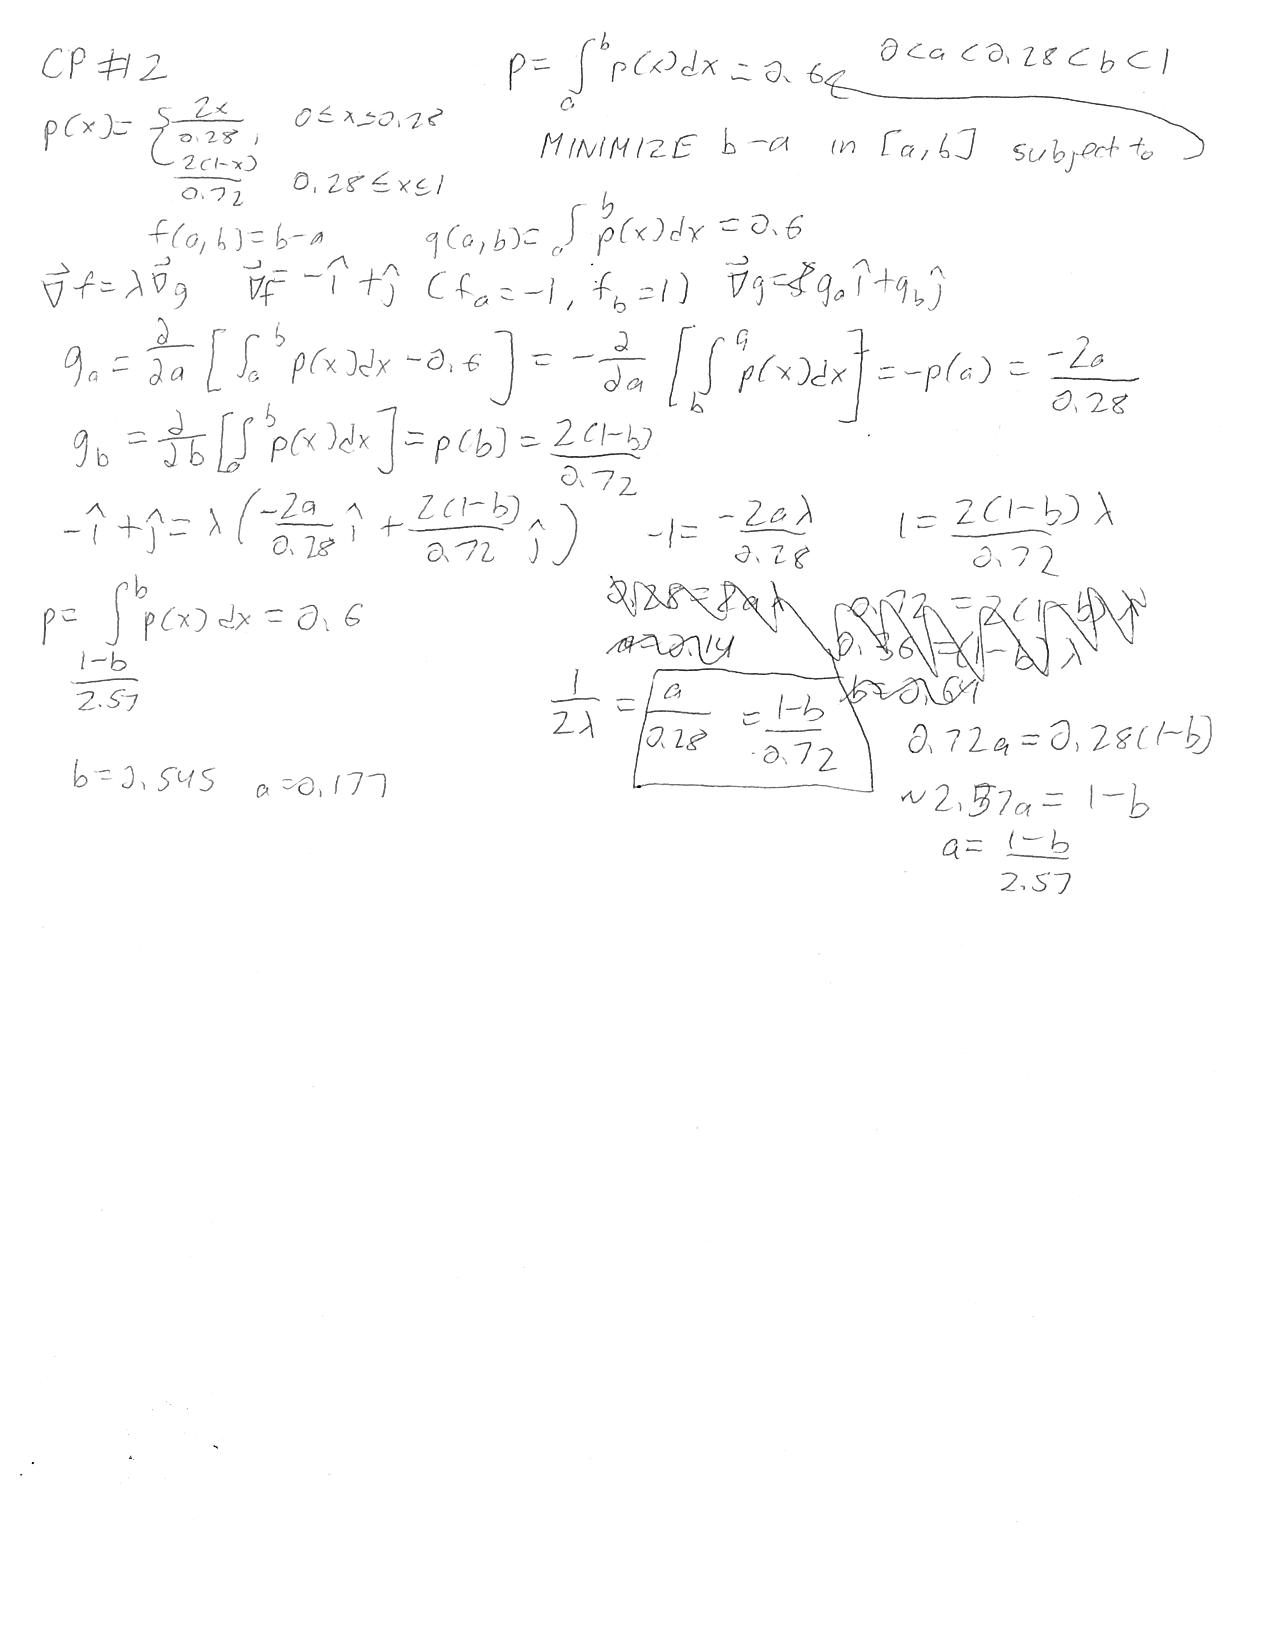
\includegraphics[]{ch 13 cp 22018-11-04-141446-1.jpg}\centering

\raggedright
\end{document}
